Lorsqu'on utilise l'implicit tiling, le client Cesium à besoin de recevoir en premier lieu une liste de tuiles disponibles. Cette liste doit lui être donnée sous forme de Subtree. Les \textit{Subtrees} dans Cesium constituent une composante essentielle pour la gestion et l'optimisation de la visualisation des données géospatiales volumineuses. Plutôt que de charger l'intégralité des données géospatiales, les Subtrees ont pour but d'indiquer au client Cesium quelles tuiles sont diponibles, quelles tuilles ont un contenu à afficher quelles sont ses enfants (\texttt{children}). Pour chacune de ces trois informations, un Subtree contient un objet \textit{Availability} (\autoref{sec:availability-class}) stockant une liste de boolean représantant chaque tuile. Pour savoir quel index de cette liste correspond à quelle tuile, un autre style de \textit{Binary Space Partitioning} est utilisé. Une \href{https://en.wikipedia.org/wiki/Z-order\_curve}{\textit{Z-order curve} ou un \textit{Morton order}}\footnote{https://en.wikipedia.org/wiki/Z-order\_curve} est utilisé pour définir les indexes (\autoref{sec:morton}).

Une fois ces Subtrees générés, il faudra les envoyer au client. Cela se fera en les transformant en JSON puis en un fichier respectant le \href{https://github.com/CesiumGS/3d-tiles/tree/main/specification/ImplicitTiling\#subtree-binary-format}{\textit{Subtree Binary Format}}\footnote{https://github.com/CesiumGS/3d-tiles/tree/main/specification/ImplicitTiling\#subtree-binary-format}

\subsection*{Hiérarchie de Subtrees}

\begin{figure}[H]
    \centering
    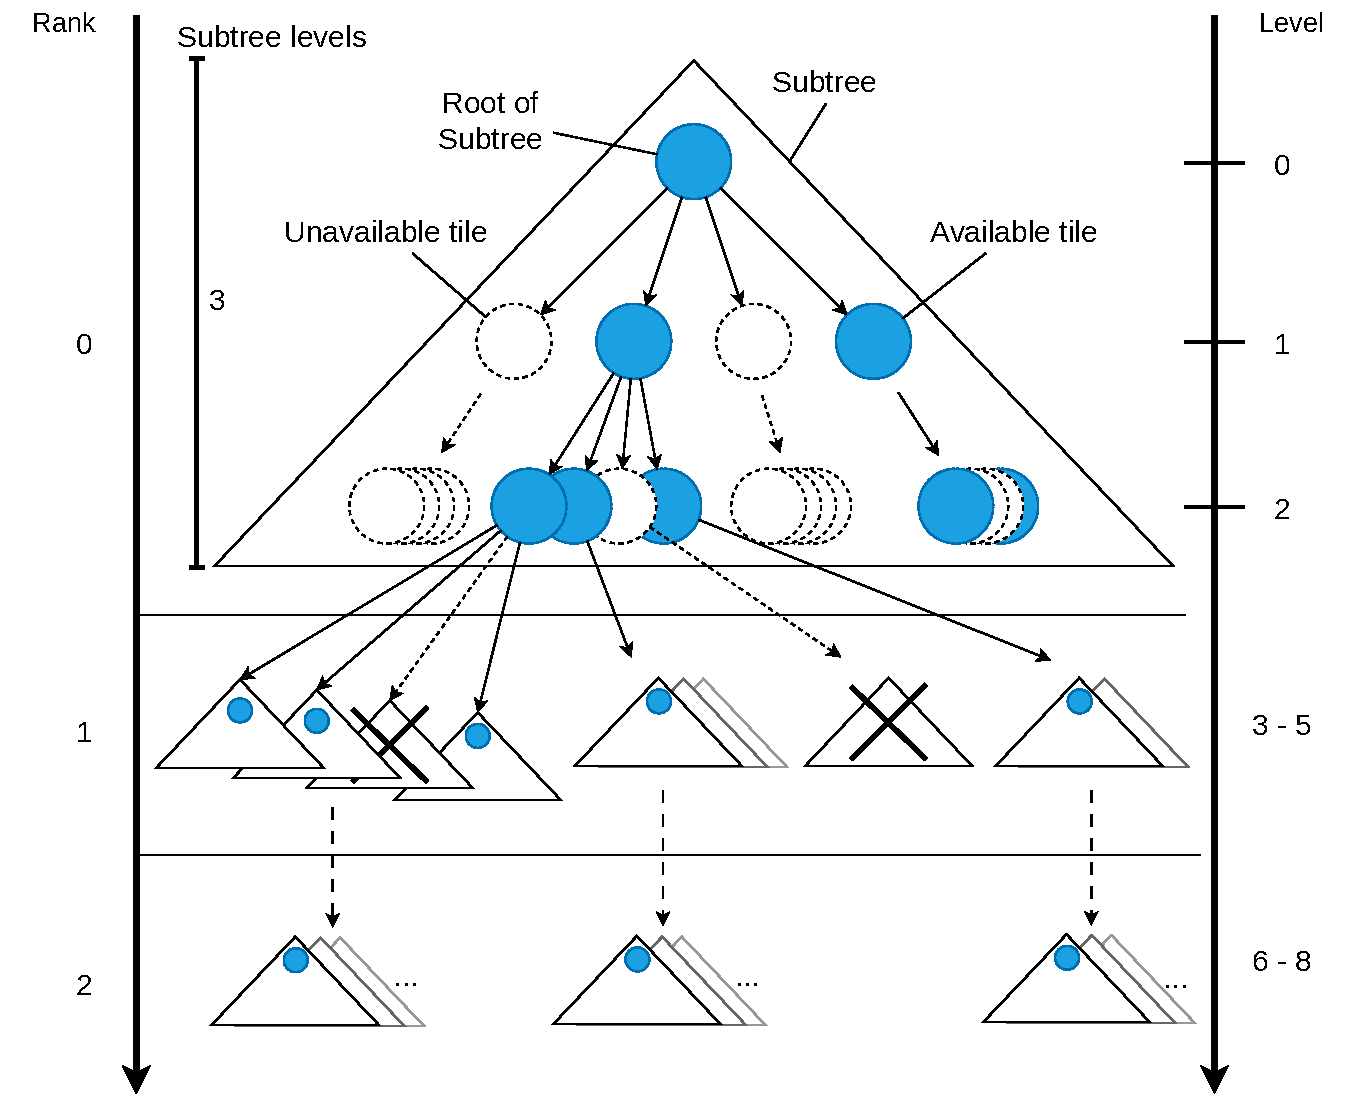
\includegraphics[width=1\textwidth]{assets/figures/Subtree_hierarchy.drawio.pdf}
    \caption{Exemple de hiérarchie de Subtrees}
    \label{fig:subtree-hierarchy}
\end{figure}

Le tileset est partitionné en Subtrees de taille \texttt{subtreeLevels} fixe. Leur schéma de subdivision suit la même logique que les tuiles d'un implicit tiling. Chaque \textit{level} ou niveau représente une subdivision de la tuile de niveau supérieur. Un Subtree est généralement de plusieurs niveau de profondeur. Chaque niveau est composé d'une liste de noeuds représentant la disponibilité d'une tuile. En fonction du shema de subdivision, quadtree ou octree, chaque noeud peut avoir 4 ou 8 enfants respectivement. On peut retrouver ces noeuds dans les listes de disponibilités citées plus haut. Les \textit{Availabilities} seront traités plus en détails dans la section \ref{sec:availability-class}.

Plusieurs Subtrees peuvent être liés entre eux pour former un arbre de Subtrees. Leur liaison se fait entre le noeud \textit{root} d'un subtree et un noeud au niveau maximum d'un autre Subtree. Par soucis de compréhension, j'appellerai le \textit{rang}, ou \textit{rank} en Anglais, d'un Subtree le niveau de profondeur de ce Subtree par rapport à la racine du tileset. Le Subtree de rang 0 est le Subtree de la racine du tileset. Les Subtree de rang maximum sont les Subtrees qui contiendront les contenus à afficher.

Finalement, quelques rêgles doivent être respectées lors d'une construction d'une hiérarchie de Subtrees:

\begin{itemize}
    \item Les Subtrees doivent être de même taille.
    \item Les Subtrees doivent avior le même schéma de subdivision.
    \item Un Subtree doit contenir au minimum un niveau.
\end{itemize}